\section{Experiments and Results}

We believe the tweets originate from soldiers and veterans can have differences with civilians on both lexical and non-lexical aspects. The experiments are divided into two parts. We first summarized the features on the large aspects to compare the difference between corpora from soldiers/veterans and civilians. Then we calculated sentiment and emotion metrics based on lexicons.

\subsection{Data Collection}

We use TWINT \citep{twint} as our data collection tool. All the data can be accessed publicly so there are no ethical considerations.

Numerous strategies considered in an attempt to procure data that belonged to the war veterans. Transcripts of podcasts and YouTube videos involving accounts of wars from the veterans, books that were written by the ex-servicemen, the public dataset that had diaries, and letters of first world war soldiers were a few sources. However, as an inference, all of these sources were highly specific to the negative aspects and impacts of war and eventually would add bias to the data.

On account of being a platform that is widely used by a large number of service-men and the civilians, Twitter was selected as the platform to extract data. Several verified Twitter pages linked to the US Army were manually analysed and a few profiles of the veterans were used as an initial set. But, we finally used the data from a verified page with the name IAVA. This is said to be the most significant association speaking to the new age of vets specifically from The United States. The profiles with a minimum of 50 tweets were only considered eligible. The final set had Twitter profiles with as few as 57 tweets and as many as 65,000 tweets. The succeeding veterans were picked by scouring through the followers of the veterans in the original set based on some keywords like the army, us-army, military in their bio.

A collection from 208 veterans profile was performed which was used for our final set of experiments. It helped us to have a dataset set of 6,61,342 tweets that were used in our analysis.

Similarly, for collection the data of civilians, we opted to chooses pages such as Netflix, USA official page, The US open and more. Here also the same guidelines were followed as in the case of finding the profiles of vets, but the only difference was that, here we were selection profiles based on keywords not similar to “army”, “us-army”, “military” in their bio. A final list of 280 civilians usernames was selected with variations in age, sex, and the number of tweets. This ultimately added 6,00,173 tweets by the general civilians and was used in our processing.

Once we had all the data that is from both the veterans and the civilians, we merged all the data to two CSV file so that is easier to process the data that we have extracted. This merged data for both were further used in our pre-processing.

\subsection{Data Process and Analysis}

\subsubsection{Lexical \& Non-Lexical Feature Summarization}

Once the data is gathered and saved in the CSV format, we then start pre-processing the gathered data after which we do our analysis where we come up with a set of results to prove our hypothesis. Sentiment analysis can be broadly categorized into two kinds, based on the type of output the analysis generates. Under our processing, we are trying to label text to be under \enquote{curses} - or bad words. Take into account the tweets of all the selected veterans from our data and then run an analysis to gather information from there. Not only this, but information such as the total counts of retweets, replies, likes, emojis, URLs, mentions and total words are calculated. Special elements in tweets can be referred to Table \ref{table:elementsRemoved}. This is one of the analysis that we are dong from the collected data.

This identical analysis is then run on tweets by ordinary people or civilians data as well. Finally, we will categorise the difference in the count of \enquote{curse} words to check the two sets of results which will ultimately help us identify an individual being in the state of depression.

The initial step we took for pre-processing our data were:

\begin{itemize}
  \item Only selecting tweets that were in English.
  \item Applying the rule to only select textual data.
\end{itemize}

It was then followed by removal of: (1) Retweets numbers; (2) Tokenizing.

Furthermore, the emojis were given a textual form so that we can get information from that part as well. This is because in this everchanging world the use of emojis has increased. These converted emojis were counted. Subsequently, profanity was predicted in the tweets.

The step to remove punctuation followed by Tokenizing which is the way toward separating a goliath string into a rundown of words. NLTK \citep{NLTK}, a python library is used for this process. Stopwords, where pull-out, as they do not change any meaning of a sentence hence, can be ignored. Tuples were generated with each word and part of speech. Finally, the counts were extracted from the tweets of both the veterans and the civilians. And was then was compared with each other.

An abstract of the process is illustrated in Figure \ref{fig:exp1}.

\begin{figure}[h]
  \centering
  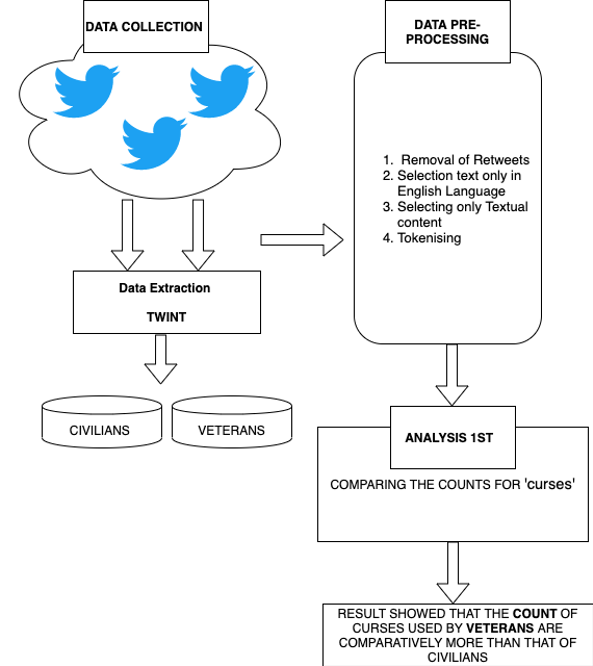
\includegraphics{images/exp1process.png}
  \caption{Process of lexical \& non-lexical feature summarization}
  \label{fig:exp1}
\end{figure}

\begin{table}[h]
  \caption{Elements to handle when preprocessing tweets}
  \label{table:elementsRemoved}
  \centering
  \renewcommand{\tabularxcolumn}{m} % we want center vertical alignment
  \begin{tabularx}{0.8\textwidth}{l  l || l  l}
    \toprule
    \textbf{Element} & \textbf{Examples} & \textbf{Element}    & \textbf{Examples}
    \tabularnewline \midrule
    URLs
                     &
    http://foo.bar   & Blank spaces      &
    \tabularnewline \hline
    Mentions to other users
                     & @Bot              & Single letter words & a b c
    \tabularnewline \hline
    Hashtags
                     & \#botRise         & Numbers             & 1994 233
    \tabularnewline \hline
    Twitter reserved words
                     & RT via            & Stopwords
                     & it I as
    \tabularnewline \bottomrule
  \end{tabularx}
\end{table}

Here is the data that was collected from the tweets (see Table \ref{table:summarized}):

\begin{table}[h]
  \caption{Summarized features from soldier and civilian corpora}
  \label{table:summarized}
  \centering
  \renewcommand{\tabularxcolumn}{m} % we want center vertical alignment
  \begin{tabularx}{0.5\textwidth}{l | l | l}
    \toprule
             & Soldiers n=208 & Civilians n=280
    \tabularnewline \hline
    tweets   & 661342         & 600173
    \tabularnewline \hline
    retweets & 869272         & 24102124
    \tabularnewline \hline
    replies  & 333204         & 5919866
    \tabularnewline \hline
    likes    & 2735134        & 123551386
    \tabularnewline \hline
    emojis   & 159583         & 69284
    \tabularnewline \hline
    urls     & 250026         & 248854
    \tabularnewline \hline
    mentions & 226533         & 325691
    \tabularnewline \hline
    words    & 51528493       & 44355619
    \tabularnewline \hline
    curses   & 28249          & 8983
    \tabularnewline \bottomrule
  \end{tabularx}
\end{table}

% \begin{itemize}
%   \item soldier stats: {'retweets': 869272, 'replies': 333204, 'likes': 2735134, 'emojis': 159583, 'urls': 250026, 'mentions': 226533, 'words': 51528493, 'curses': 28249, 'tweets': 661342}
%   \item civilian stats: {'retweets': 24102124.0, 'replies': 5919866.0, 'likes': 123551386, 'emojis': 69284, 'urls': 248854, 'mentions': 325691, 'words': 44355619, 'curses': 8983, 'tweets': 600173}
% \end{itemize}

\subsubsection{Sentiment \& Emotion Analysis}

Tweets are filtered and only tweets with texts originate from users themselves remain, which means the likes and retweets are filtered.

The corpora are then pre-processed to remove elements mentioned in Table \ref{table:elementsRemoved}.

We try not to remove punctuations and stopwords because we need to do Part-of-Speech (POS) tagging after tokenizing. Both tokenizing and POS tagging is done by NLTK \citep{NLTK}.

We use lexicons to score the words in our corpora. SentiWordNet is used for sentiment polarity analysis and NRC Word-Emotion Association Lexicon (EmoLex) \citep{Mohammad13} based on the model of Plutchik’s wheel of emotions \citep{plutchik2003emotions} (see Figure \ref{fig:wheel}, with additional Positiveness and Negativeness) is for emotion analysis.

\begin{figure}[h]
  \centering
  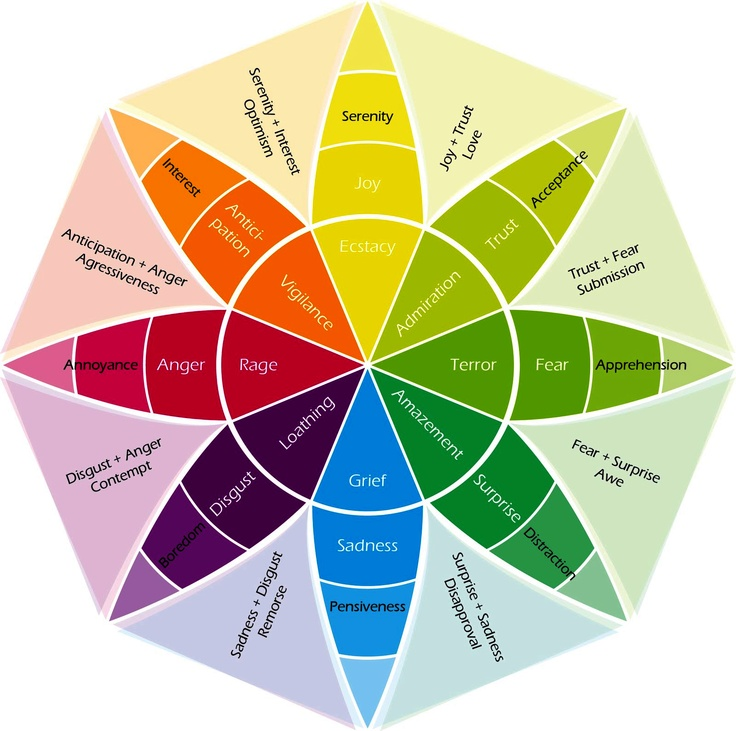
\includegraphics[width=0.8\textwidth]{images/wheel-of-emotions.jpg}
  \caption{Plutchik’s wheel of emotions}
  \label{fig:wheel}
\end{figure}

Once the POS tags of words are generated. We search the synonyms of words in SentiWordNet to determine the scoring for positiveness, negativeness and objectiveness by calculating means among synonyms. Meanwhile, EmoLex is used to perform emotion analysis on 10 emotions. Scores of one tweet are generated calculating the means of the scores of all the words after preprocessing.

The result data obtained by applying SentiWordNet is shown in Table \ref{table:sentiResult}.
The result produced by using EmoLex is shown in Table \ref{table:emolexResult}.

We also counted adjectives with top 100 frequencies in soldiers and civilians corpora, for we think that adjectives have more subjective meanings than verbs, nouns, etc. We discovered some words with more \enquote{political} meanings appear to be different in the lists of two corpora. The list of adjectives is shown in Table \ref{table:wordsComparison}.


\begin{table}[h]
  \caption{Results of sentiment analysis using SentiWordNet}
  \label{table:sentiResult}
  \centering
  \renewcommand{\tabularxcolumn}{m} % we want center vertical alignment
  \begin{tabularx}{\textwidth}{l l | l l l l l}
    \toprule
              &      & \textbf{Valid Cnt.} & \textbf{Valid Len.} & \textbf{Positive.}     & \textbf{Negative}      & \textbf{Objective.}
    \tabularnewline \midrule
    Soldiers  & Mean & 3179.54*            & 16.450              & 257.58$\times 10^{-4}$ & 196.10$\times 10^{-4}$ & 3371.7$\times 10^{-4}$
    \tabularnewline
    n=208     & Std. & 5041.70             & 6.6427              & 78.586$\times 10^{-4}$ & 64.386$\times 10^{-4}$ & 750.49$\times 10^{-4}$
    \tabularnewline \hline \hline
    Civilians & Mean & 2143.66*            & 14.293              & 262.65$\times 10^{-4}$ & 177.39$\times 10^{-4}$ & 3530.5$\times 10^{-4}$
    \tabularnewline
    n=280     & Std. & 5286.12             & 5.2067              & 87.432$\times 10^{-4}$ & 64.786$\times 10^{-4}$ & 720.09$\times 10^{-4}$
    \tabularnewline \bottomrule
  \end{tabularx}
\end{table}


\begin{table}[h]
  \caption{Results of emotion analysis using EmoLex}
  \label{table:emolexResult}
  \centering
  \renewcommand{\tabularxcolumn}{m} % we want center vertical alignment
  \begin{tabularx}{\textwidth}{l l l l l l}
    \toprule
    Soldiers: n=208
    \tabularnewline \midrule
     & \textbf{Trust}+   & \textbf{Anger}+ & \textbf{Surprise}    & \textbf{Joy}      & \textbf{Positive.}
    \tabularnewline \midrule
    Mean $\times 10^{-4}$
     & 422.84            & 167.17          & 149.99               & 312.51            & 637.50
    \tabularnewline
    Std. $\times 10^{-4}$
     & 154.94            & 83.143          & 62.113               & 151.64            & 213.55
    \tabularnewline \midrule
     & \textbf{Disgust}+ & \textbf{Fear}+  & \textbf{Anticipat.}  & \textbf{Sadness}+ & \textbf{Negative.}+
    \tabularnewline \midrule
    Mean$\times 10^{-4}$
     & 122.09            & 193.43          & 295.57               & 149.34            & 339.61
    \tabularnewline
    Std.$\times 10^{-4}$
     & 74.795            & 89.380          & 112.40               & 66.053            & 148.79
    \tabularnewline \hline \hline
    Civilians: n=280
    \tabularnewline \midrule
     & \textbf{Trust}    & \textbf{Anger}  & \textbf{Surprise}+   & \textbf{Joy}+     & \textbf{Positive.}+
    \tabularnewline \midrule
    Mean $\times 10^{-4}$
     & 399.72            & 132.03          & 163.72               & 349.44            & 650.63
    \tabularnewline
    Std.$\times 10^{-4}$
     & 170.45            & 80.189          & 108.13               & 224.58            & 269.03
    \tabularnewline \midrule
     & \textbf{Disgust}  & \textbf{Fear}   & \textbf{Anticipat.}+ & \textbf{Sadness}  & \textbf{Negative.}
    \tabularnewline \midrule
    Mean$\times 10^{-4}$
     & 98.934            & 163.78          & 330.09               & 131.82            & 283.00
    \tabularnewline
    Std.$\times 10^{-4}$
     & 82.884            & 108.23          & 152.86               & 87.180            & 160.08
    \tabularnewline \bottomrule
  \end{tabularx}
\end{table}


\begin{table}[h]
  \caption{List of \enquote{political} adjectives with rankings and frequencies}
  \label{table:wordsComparison}
  \centering
  \renewcommand{\tabularxcolumn}{m} % we want center vertical alignment
  \begin{tabularx}{0.8\textwidth}{l | l | l || l | l | l}
    \toprule
    \textbf{Word} & \textbf{Soldiers} & \textbf{Civilians} & \textbf{Word} & \textbf{Soldiers} & \textbf{Civilians}
    \tabularnewline \midrule
    military      & 4.46 (17th)       & -                  & dead          & 1.20 (77th)       & -
    \tabularnewline \hline
    american      & 3.85 (24th)       & 1.20 (79th)        & human         & 1.17 (80th)       & 1.01 (91st)
    \tabularnewline \hline
    political     & 2.12 (40th)       & -                  & local         & 1.16 (81st)       & 1.26 (72nd)
    \tabularnewline \hline
    medical       & 1.75 (47th)       & -                  & democratic    & 1.15 (83rd)       & -
    \tabularnewline \hline
    public        & 1.56 (51st)       & 1.32 (68th)        & illegal       & 1.14* (85th)      & -
    \tabularnewline \hline
    social        & 1.44 (60th)       & 1.78 (51st)        & foreign       & 1.14* (85th)      & -
    \tabularnewline \hline
    sick          & 1.37 (64th)       & -                  & poor          & 1.10 (90th)       & -
    \tabularnewline \hline
    personal      & 1.31 (71st)       & 1.21 (78th)        & republican    & 1.07 (93rd)       & -
    \tabularnewline \bottomrule
  \end{tabularx}
\end{table}
